\chapter{理論・関連研究}
\label{chap:theory_related_work}

本章では，本研究に関連する一般的な理論的背景を整理する．

まず，記号と問題設定を整理し，系列モデル（Transformer），潜在変数モデル（AE/VAE），対照学習の基礎をまとめる．
続いて，動作表現学習と言語空間の接続（MotionCLIP）を述べ，最後に強化学習の基礎とロボットナビゲーション関連研究（VLA，NaVILA）を紹介する．

\section{記号と問題設定}
\label{sec:notation_problem}

\paragraph{動作データ}\leavevmode\\

2D 関節系列を
\begin{align}
  X \in \mathbb{R}^{T \times J \times 2}
\end{align}
と表す．ここで $T$ はフレーム長，$J$ は関節数である．
フレーム $t$ における関節 $j$ の 2D 座標を $x_{t,j}\in\mathbb{R}^2$ とし，
\begin{align}
  X = \{x_{t,j}\}_{t=1..T,\ j=1..J}
\end{align}
と書く．

\paragraph{言語データ}\leavevmode\\

テキスト列 $w$ に対し，テキストエンコーダ $e_{\mathrm{text}}(\cdot)$ により
\begin{align}
  u_{\mathrm{sem}} = e_{\mathrm{text}}(w) \in \mathbb{R}^{D_{\mathrm{sem}}}
\end{align}
を得る．類似度計算のために L2 正規化 $\mathrm{normalize}(x)=x/\|x\|_2$ を用いる場合は
\begin{align}
  \tilde{u}_{\mathrm{sem}}=\mathrm{normalize}(u_{\mathrm{sem}})
\end{align}
と書く．

\paragraph{潜在表現}\leavevmode\\

潜在表現を $z\in\mathbb{R}^{D}$ と表す．生成モデルや表現学習では，低次元の潜在表現を介して
高次元の系列や意味表現を扱うことが多い．

\section{ニューラルネットワークアーキテクチャ}
\label{sec:NN_Arch}

\subsection{Transformer}
\label{subsec:Transformer}
Transformer \cite{Transformer} は，系列データの表現力を保ちながら，
RNN の逐次計算に由来する並列化の難しさを解消するために提案された．
当時主流の RNN ベース encoder--decoder は，時刻 $t$ の計算に $t-1$ の結果が必要で，
学習・推論ともに並列化が困難であった．
また系列が長くなるほど計算効率が低下し，長距離依存の学習も難しくなる．
Transformer は注意機構のみでトークン間依存をモデル化し，
系列全体を行列演算として同時に扱うことで高い並列性を得る．
本節の概説は\cite{kikuta2025genai} を参考に整理した．

\begin{figure}[htbp]
  \centering
  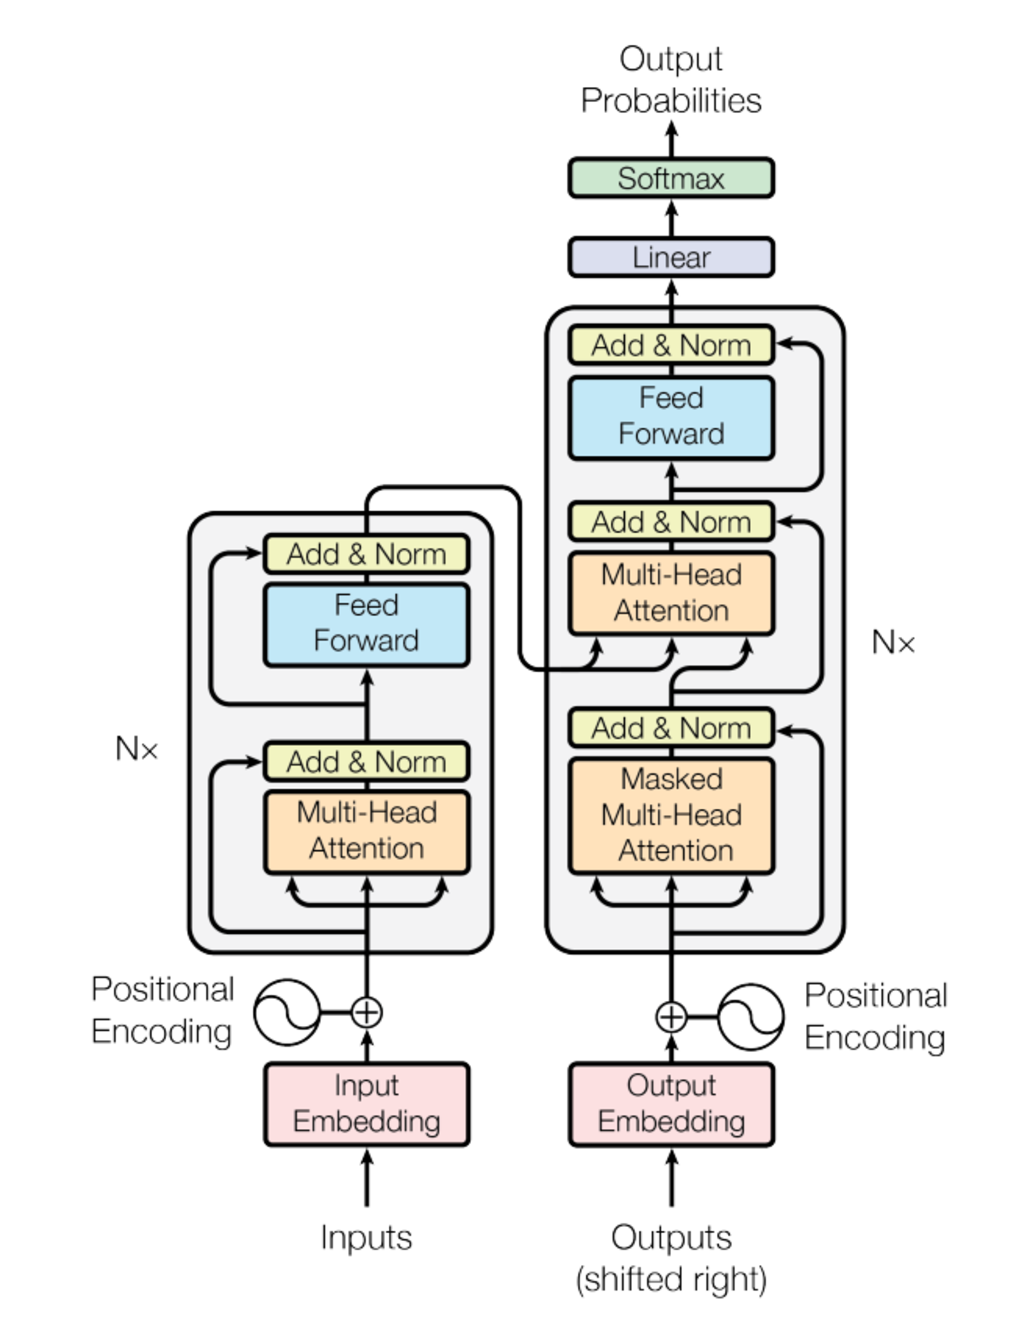
\includegraphics[width=1.0\linewidth]{figs/2/transformer_model.pdf}
  \caption{Transformer のアーキテクチャ（\cite{Transformer}より引用）}
  \label{fig:transformer}
\end{figure}

図\ref{fig:transformer}に示すように，Transformer はエンコーダとデコーダから構成される．
エンコーダは入力系列 $X$ を文脈化表現へ写像し，
デコーダは自己注意（Self-Attention）とエンコーダ出力への注意（Cross-Attention）により
出力系列を生成する \cite{Transformer}．
各層は Multi-Head Attention（MHA）と Position-wise Feed-Forward Network（FFN）からなり，
各サブレイヤに残差接続と Layer Normalization を適用して安定化する．
Self-Attention は順序情報を明示的に持たないため，
入力埋め込みには位置情報を付与する Positional Encoding を加える \cite{Transformer}．

以下では Self-Attention を中心に数式で定義する．
入力系列を $X\in\mathbb{R}^{n\times d_{\mathrm{model}}}$（$n$ トークン，埋め込み次元 $d_{\mathrm{model}}$）とする．
ここで $d_k$ と $d_v$ は各ヘッドの key/value 次元，$H$ はヘッド数であり，
一般に $d_k=d_v=d_{\mathrm{model}}/H$ を用いる．
線形写像により
\begin{align}
  Q=XW^Q,\quad K=XW^K,\quad V=XW^V
\end{align}
を作る（$W^Q,W^K,W^V\in\mathbb{R}^{d_{\mathrm{model}}\times d_k}$）．
Scaled Dot-Product Attention を
\begin{align}
  \mathrm{Attention}(Q,K,V)
  = \mathrm{softmax}\!\left(\frac{QK^\top}{\sqrt{d_k}}\right)V
\end{align}
で定義する \cite{Transformer}．
ここで $\frac{1}{\sqrt{d_k}}$ は内積のスケールを正規化し，
softmax の飽和を緩和するために導入される．
なおデコーダの自己注意では，将来トークンへの参照を防ぐために因果マスクを適用することが一般的である \cite{Transformer}．

\paragraph{Multi-Head Attention}
ヘッド数を $H$ とするとき，各ヘッド $h$ で
\begin{align}
  \mathrm{head}_h
  = \mathrm{Attention}\!\left(XW_h^Q,\ XW_h^K,\ XW_h^V\right)
\end{align}
を計算し，結合して
\begin{align}
  \mathrm{MHA}(X)
  = \mathrm{Concat}(\mathrm{head}_1,\dots,\mathrm{head}_H)W^O
\end{align}
とする（$W^O\in\mathbb{R}^{Hd_v\times d_{\mathrm{model}}}$）\cite{Transformer}．
複数ヘッドにより，異なる部分空間における依存関係を並列に捉えることができる．

\paragraph{Position-wise Feed-Forward Network}
各トークンに独立に適用する 2 層 MLP を
\begin{align}
  \mathrm{FFN}(x)=\sigma(xW_1+b_1)W_2+b_2
\end{align}
で表す（$\sigma$ は ReLU 等）\cite{Transformer}．
注意機構がトークン間の情報集約を担うのに対し，
FFN は各トークン表現の非線形変換を担う．

\paragraph{Residual と LayerNorm}
Transformer ブロックはサブレイヤ $\mathrm{Sublayer}(\cdot)$ に対して
\begin{align}
  \mathrm{AddNorm}(x)=\mathrm{LayerNorm}\bigl(x+\mathrm{Sublayer}(x)\bigr)
\end{align}
の形で安定化される \cite{Transformer}．

\paragraph{Positional Encoding}
トークン位置 $p$ と次元 index $i$ に対し，正弦波位置埋め込みは
\begin{align}
  \mathrm{PE}(p,2i)   & = \sin\left(p/10000^{2i/d_{\mathrm{model}}}\right), \\
  \mathrm{PE}(p,2i+1) & = \cos\left(p/10000^{2i/d_{\mathrm{model}}}\right)
\end{align}
で与えられる \cite{Transformer}．
動作系列に対しても，フレーム時刻（時間ステップ）を位置 $p$ とみなすことで同様に適用できる．

本研究では Transformer を MotionCLIP のエンコーダ／デコーダとして用い，
2D 歩容系列から動作潜在を抽出し，テキスト意味埋め込みとの整合を学習する．
詳細は動作と言語の接続（\ref{sec:motion_language_alignment}）および提案手法（第\ref{chap:proposed_method}章）で述べる．


\section{オートエンコーダと潜在変数モデル}
\label{sec:latent_models}

本節では，高次元データを低次元の潜在表現で扱うための代表的手法として，
変分オートエンコーダ（VAE）を整理する．

\subsection{変分オートエンコーダ（VAE）}
\label{subsec:VAE}

VAE は潜在変数 $z$ を確率変数として扱い，データ生成過程を
「まず事前分布 $p(z)$ から $z$ をサンプルし，その後 $p_\theta(X\mid z)$ から $X$ を生成する」
という生成モデルとして定式化する．
潜在次元を $D$ とし，結合分布を
\begin{align}
  p_\theta(X,z)=p_\theta(X\mid z)p(z)
\end{align}
とする．一般に事前分布として
\begin{align}
  p(z)=\mathcal{N}(0,I)
\end{align}
を用いる（$I$ は $D$ 次元単位行列）．
このとき周辺尤度は
\begin{align}
  \log p_\theta(X) = \log\int p_\theta(X\mid z)p(z)\,dz
\end{align}
で与えられるが，積分が高次元となるため直接最大化することは困難である．
そこで近似事後分布 $q_\phi(z\mid X)$（推論モデル；エンコーダに対応）を導入し，
Jensen の不等式により ELBO（Evidence Lower Bound）
\begin{align}
  \log p_\theta(X)
  \ge
  \mathbb{E}_{q_\phi(z\mid X)}[\log p_\theta(X\mid z)]
  -\mathrm{KL}\bigl(q_\phi(z\mid X)\,\|\,p(z)\bigr)
  \label{eq:elbo}
\end{align}
を最大化する \cite{VAE}．
右辺第1項は「$z$ から $X$ をうまく復元（生成）できる」ことを促す再構成項であり，
観測モデルの仮定に依存する（例えばガウス尤度を仮定すれば L2 損失に対応する）．
第2項は近似事後 $q_\phi(z\mid X)$ を事前 $p(z)$ に近づける正則化項として働く．
実装上は負の ELBO を損失とし，
\begin{align}
  \mathcal{L}_{\mathrm{VAE}}=
  -\mathbb{E}_{q_\phi(z\mid X)}[\log p_\theta(X\mid z)]
  +\mathrm{KL}\bigl(q_\phi(z\mid X)\,\|\,p(z)\bigr)
\end{align}
を最小化する．
この枠組みにより，学習後は $z\sim p(z)$ をサンプリングしデコーダを通すことで，新しいデータを生成できる．

\paragraph{再パラメータ化トリック}
VAE の学習では期待値項 $\mathbb{E}_{q_\phi(z\mid X)}[\cdot]$ が現れるが，
$z$ を直接サンプルすると勾配推定が高分散になりやすい．
そこで $q_\phi(z\mid X)$ を
\begin{align}
  q_\phi(z\mid X)=\mathcal{N}\!\bigl(\mu_\phi(X),\mathrm{diag}(\sigma_\phi^2(X))\bigr)
\end{align}
とし（$\sigma_\phi$ は標準偏差），
\begin{align}
  z=\mu_\phi(X)+\sigma_\phi(X)\odot\epsilon,\quad \epsilon\sim\mathcal{N}(0,I)
\end{align}
と書き換える．
これにより確率性を $\epsilon$ に押し込み，$z$ を $\mu_\phi,\sigma_\phi$ の決定論的関数として表せるため，
期待値項をモンテカルロ近似しつつ勾配に基づく最適化が可能となる \cite{VAE}．

\paragraph{KL項の閉形式}
$q=\mathcal{N}(\mu,\mathrm{diag}(\sigma^2))$，$p=\mathcal{N}(0,I)$ のとき，
KL ダイバージェンスは
\begin{align}
  \mathrm{KL}(q\|p)
  = \frac{1}{2}\sum_{k=1}^{D}\left(\mu_k^2+\sigma_k^2-\log\sigma_k^2-1\right)
  \label{eq:kl_gaussian}
\end{align}
と閉形式で計算できる．
このため VAE は KL 項の推定が安定しやすく，学習を実装しやすいという利点がある．




\section{対照学習}
\label{sec:contrastive}

対照学習は，埋め込み空間上で「意味的に対応する正例」を近づけ，
「対応しない負例」を遠ざけることで表現を学習する枠組みである．
自己教師ありではデータ拡張によって同一サンプルから正例対を作り，
教師ありでは同一ラベルのサンプルを正例として扱う \cite{supcon}．
実装上は，バッチ内の他サンプルを負例とみなし，
正例を当てる分類問題（InfoNCE 形式）として損失を構成することが多い \cite{clip}．
以下では温度付き正規化を導入した上で，CLIP/SigLIP/SupCon の代表的な定式化を示す．
対照学習および CLIP の説明は\cite{kikuta2025genai} を参考に整理した．

\subsection{温度付き正規化とコサイン類似度}
\label{subsec:cosine_temp}

埋め込み $a,b$ を L2 正規化すると
\begin{align}
  \tilde{a}=\frac{a}{\|a\|_2},\quad \tilde{b}=\frac{b}{\|b\|_2}
\end{align}
であり，コサイン類似度は内積に一致する：
\begin{align}
  \cos(a,b)=\tilde{a}^\top \tilde{b}.
\end{align}
対照学習では温度 $\tau>0$ を用いて logit を $s/\tau$ とし，
分布の鋭さ（勾配のスケール）を調整することが一般的である．

\subsection{CLIP の損失（画像--言語の双方向分類としての定式化）}
\label{subsec:CLIP_loss}

CLIP \cite{clip} は，バッチ内の $N$ 個の画像--テキスト対応 $(I_i,T_i)$ を用い，
画像エンコーダ $f_I$ とテキストエンコーダ $f_T$ の出力を
\begin{align}
  v_i = \mathrm{normalize}(f_I(I_i)),\quad
  t_i = \mathrm{normalize}(f_T(T_i))
\end{align}
とする．類似度行列（logits）を
\begin{align}
  \ell_{ij} = \frac{v_i^\top t_j}{\tau}
\end{align}
で定義する．実装では logit scale $\exp(\gamma)$ を学習し，
$\ell_{ij}=\exp(\gamma)\,v_i^\top t_j$ とすることも多く，$\tau$ はその逆数に相当する \cite{clip}．
正解ラベルを $y_i=i$ としたとき，画像$\rightarrow$テキストのクロスエントロピー
\begin{align}
  \mathcal{L}_{I\rightarrow T}
  = -\frac{1}{N}\sum_{i=1}^{N}\log
  \frac{\exp(\ell_{ii})}{\sum_{j=1}^{N}\exp(\ell_{ij})}
\end{align}
およびテキスト$\rightarrow$画像
\begin{align}
  \mathcal{L}_{T\rightarrow I}
  = -\frac{1}{N}\sum_{i=1}^{N}\log
  \frac{\exp(\ell_{ii})}{\sum_{j=1}^{N}\exp(\ell_{ji})}
\end{align}
を計算する \cite{clip}．最終損失は
\begin{align}
  \mathcal{L}_{\mathrm{CLIP}}=\frac{1}{2}\left(\mathcal{L}_{I\rightarrow T}+\mathcal{L}_{T\rightarrow I}\right)
  \label{eq:clip_loss}
\end{align}
である \cite{clip}．
この定式化により，バッチ内で「正例を当てる分類問題」として対照学習が実装できる．

\subsection{SigLIP の損失（Sigmoid Loss）}
\label{subsec:SigLIP_loss}

SigLIP \cite{siglip} は softmax 正規化に依存せず，画像--テキストの全組み合わせに対して
シグモイド型の対照損失を用いる枠組みを提案する．
バッチ内ペア $(I_i,T_j)$ のスコアを $s_{ij}=v_i^\top t_j/\tau$ とし，
一致ラベルを $y_{ij}\in\{+1,-1\}$（$i=j$ なら $+1$，それ以外は $-1$）とすると，
対数シグモイドに基づく損失は
\begin{align}
  \mathcal{L}_{\mathrm{SigLIP}}
  = -\frac{1}{N^2}\sum_{i=1}^{N}\sum_{j=1}^{N}\log \sigma\!\left(y_{ij}\, s_{ij}\right)
  \label{eq:siglip_loss}
\end{align}
と書ける \cite{siglip}（$\sigma(\cdot)$ はシグモイド関数）．
ここでは等重みの基本形を示し，実装によっては $y\in\{0,1\}$ の BCE 形式や
正例・負例の重み付けを用いる場合がある．

\subsection{教師あり対照学習（SupCon）}
\label{subsec:SupCon}

教師あり対照学習（Supervised Contrastive Learning: SupCon）\cite{supcon} は，
同一クラス（同一ラベル）のサンプルを正例として扱う．
バッチ index 集合を $I$，アンカー $i$ の正例集合を
\begin{align}
  P(i)=\{p\in I\mid y_p=y_i,\ p\neq i\}
\end{align}
とし，$\tilde{z}_i=\mathrm{normalize}(f(x_i))$ を正規化済み埋め込みとする．
正例が存在するアンカー集合を $I^+=\{i\in I\mid |P(i)|>0\}$ とすると，
SupCon の損失は
\begin{align}
  \mathcal{L}_{\mathrm{SupCon}}
  = \frac{1}{|I^+|}\sum_{i \in I^+}\frac{-1}{|P(i)|}\sum_{p\in P(i)}
  \log \frac{\exp(\tilde{z}_i^\top \tilde{z}_p/\tau)}{\sum_{a\in I\setminus\{i\}}\exp(\tilde{z}_i^\top \tilde{z}_a/\tau)}
  \label{eq:supcon_loss}
\end{align}
で与えられる \cite{supcon}．
同一クラスの埋め込みを近づけ，異なるクラスを分離する効果を持つ．


\section{動作表現学習と言語空間の接続}
\label{sec:motion_language_alignment}

前節で述べた対照学習の枠組みは，画像--テキストの対応関係を学習するために設計されたものであるが，
この枠組みを動作（モーション）ドメインに拡張することで，
テキストによる動作生成や編集が可能となる．
本節では，Tevet ら \cite{MotionCLIP} が提案した \textbf{MotionCLIP} について整理する．
MotionCLIP は動作表現を CLIP 空間に整列させることで，
テキストから動作を生成する Text-to-Motion を実現する手法である．

\subsection{MotionCLIP の概要}
\label{subsec:motion_clip_alignment}

動作生成において，意味的に構造化された潜在空間を獲得することは重要な課題である．
CLIP \cite{clip} は大規模な画像--テキストペアで学習されており，
その潜在空間は意味的に滑らかで，分離性が高いことが知られている．
MotionCLIP はこの性質をモーションデータにも転移するため，
動作オートエンコーダの潜在空間を CLIP の潜在空間に整列させる．

動作系列を $p_{1:T}$ とし，各フレーム $p_i \in \mathbb{R}^{J \times 6}$ は
$J$ 個の関節の 6D 回転表現を含むとする．
Transformer ベースのエンコーダ $E$ とデコーダ $D$ を用いて，
\begin{align}
  z_p = E(p_{1:T}), \quad \hat{p}_{1:T} = D(z_p)
\end{align}
と定義する．ここで $z_p \in \mathbb{R}^{D_{\mathrm{CLIP}}}$ は CLIP 空間と同次元の潜在表現である．

図\ref{fig:motionclip_auto_encoder}に MotionCLIP のオートエンコーダ構成を示す．
Transformer エンコーダはフレーム列とプレフィックス・トークンから潜在を抽出し，
デコーダはその潜在から系列を復元する \cite{MotionCLIP}．

\paragraph{Transformer エンコーダ}
動作系列 $p_{1:T}$ を Transformer エンコーダに入力する際，
各フレームを線形射影で埋め込み次元に変換し，位置埋め込みを加算する．
さらに，学習可能なプレフィックス・トークン $z_{\mathrm{tk}}$ を先頭に追加し，
Transformer の出力のうち最初のトークンに対応する部分を潜在表現 $z_p$ として取り出す：
\begin{align}
  z_p = E(z_{\mathrm{tk}}, p_{1:T}).
\end{align}

\paragraph{Transformer デコーダ}
デコーダは潜在表現 $z_p$ を key および value として受け取り，
query には位置符号化 $\mathrm{PE}(1:T)$ を用いる．
各時刻の出力を線形射影でポーズ空間に変換し，動作系列を復元する：
\begin{align}
  \hat{p}_{1:T} = D(z_p).
\end{align}

\begin{figure}[htbp]
  \centering
  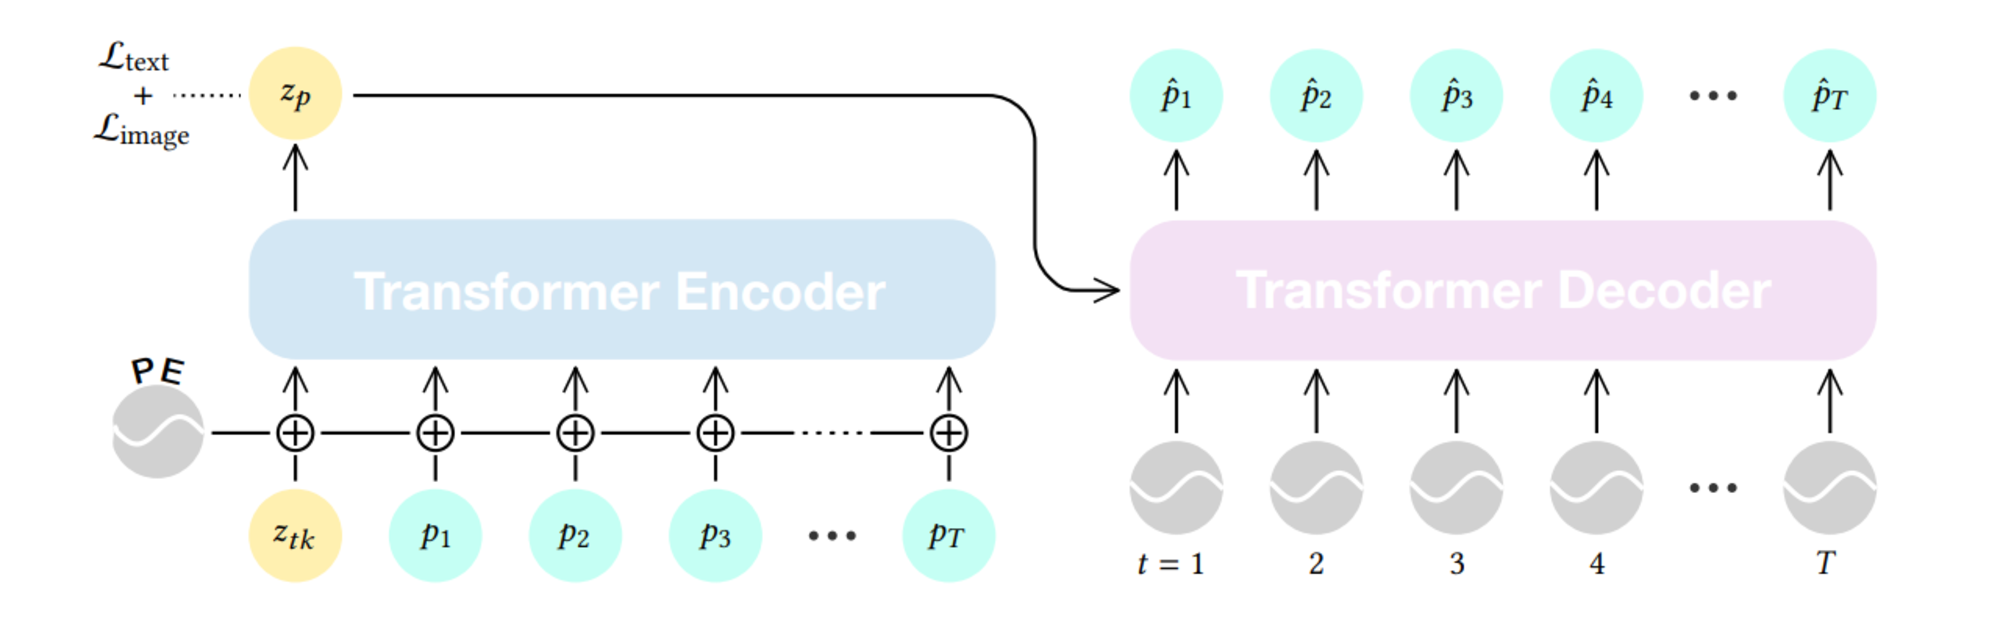
\includegraphics[width=\textwidth]{figs/2/motionclip_auto_encoder.pdf}
  \caption{MotionCLIP のオートエンコーダの構造（\cite{MotionCLIP}より引用）}
  \label{fig:motionclip_auto_encoder}
\end{figure}

\subsection{MotionCLIP の損失関数}
\label{subsec:motionclip_loss}

MotionCLIP の学習では，再構成損失に加えて CLIP 空間への整列損失を用いる．

\paragraph{再構成損失}
本研究では 2D 関節系列のみを扱うため，関節角度やメッシュ頂点位置の項は用いず，
2D 関節座標の再構成誤差と速度（フレーム差分）の誤差のみを最小化する：
\begin{align}
  \mathcal{L}_{\mathrm{recon}}
   & = \frac{1}{JT}\sum_{t=1}^{T}\sum_{j=1}^{J}\|x_{t,j} - \hat{x}_{t,j}\|^2 \notag \\
   & \quad + \frac{1}{J(T-1)}\sum_{t=1}^{T-1}\sum_{j=1}^{J}
  \|(x_{t+1,j}-x_{t,j})-(\hat{x}_{t+1,j}-\hat{x}_{t,j})\|^2
  \label{eq:motionclip_recon}
\end{align}
ここで $x_{t,j}\in\mathbb{R}^2$ はフレーム $t$ における関節 $j$ の 2D 座標である．

\paragraph{テキスト損失}
動作にテキストラベル $t$ が付与されている場合，
CLIP のテキストエンコーダ $\mathrm{CLIP}_{\mathrm{text}}$ を用いて，
動作の潜在表現をテキスト埋め込みに近づける：
\begin{align}
  \mathcal{L}_{\mathrm{text}} = 1 - \cos\bigl(\mathrm{CLIP}_{\mathrm{text}}(t),\, z_p\bigr).
  \label{eq:motionclip_text}
\end{align}

\paragraph{画像損失}
動作系列から単一フレームをレンダリングして合成画像 $s$ を生成し，
CLIP の画像エンコーダ $\mathrm{CLIP}_{\mathrm{image}}$ を用いて整列を強化する：
\begin{align}
  \mathcal{L}_{\mathrm{image}} = 1 - \cos\bigl(\mathrm{CLIP}_{\mathrm{image}}(s),\, z_p\bigr).
  \label{eq:motionclip_image}
\end{align}
この自己教師あり画像損失により，テキストラベルでは捉えきれない細かな動作特徴の整列が可能となる．

\paragraph{全体損失}
最終的な損失関数は以下で定義される：
\begin{align}
  \mathcal{L} = \mathcal{L}_{\mathrm{recon}} + \lambda_{\mathrm{text}}\mathcal{L}_{\mathrm{text}} + \lambda_{\mathrm{image}}\mathcal{L}_{\mathrm{image}}
  \label{eq:motionclip_total}
\end{align}
ここで $\lambda_{\mathrm{text}}, \lambda_{\mathrm{image}}$ は整列損失の重み係数である．

\subsection{MotionCLIP による Text-to-Motion 生成}
\label{subsec:text_to_motion}

学習済み MotionCLIP を用いた Text-to-Motion 生成は，以下の手順で行われる：
\begin{enumerate}
  \item 入力テキスト $t$ を CLIP テキストエンコーダで埋め込む：$z_t = \mathrm{CLIP}_{\mathrm{text}}(t)$
  \item 得られた埋め込み $z_t$ を動作デコーダに入力：$\hat{p}_{1:T} = D(z_t)$
\end{enumerate}
動作の潜在空間が CLIP 空間に整列されているため，
CLIP テキストエンコーダの出力を直接デコーダに渡すことで動作生成が可能となる．

この枠組みの利点は，CLIP が持つ豊富な意味的知識を動作ドメインに転移できる点にある．
訓練時に見ていない動作記述（例：「ウサイン・ボルト」「白鳥の湖」）であっても，
CLIP の埋め込み空間における類似性を介して，意味的に妥当な動作を生成できる可能性がある．

\subsection{MotionCLIP の潜在空間の性質}
\label{subsec:latent_space_properties}

MotionCLIP により CLIP 空間に整列された動作潜在空間は，以下の性質を持つことが期待される：
\begin{itemize}
  \item \textbf{滑らかさ（Smoothness）}：
        意味的に類似した動作は潜在空間で近くに配置され，
        2 つの動作間の線形補間が意味的に妥当な中間動作を生成する．
  \item \textbf{分離性（Disentanglement）}：
        動作の異なる属性（例：上半身と下半身の動き，スタイル）が潜在空間で独立した方向に符号化され，
        潜在空間での加減算による編集が可能となる．
  \item \textbf{意味的構造（Semantic Structure）}：
        動作の潜在表現とテキストの埋め込みとの類似度計算により，
        動作認識タスクにも適用可能となる．
\end{itemize}

これらの性質は，MotionCLIP が CLIP 空間の持つ構造を動作ドメインに継承することで実現される．


\section{強化学習（Actor-Critic，GAE，PPO）}
\label{sec:RL}

強化学習は，環境との相互作用を通じて累積報酬を最大化する方策を学習する枠組みであり，
最適制御に近い問題設定を持つ一方で，教師信号が逐次的な報酬としてのみ観測される点が特徴である．
本研究では連続制御の歩行方策を対象とするため，方策勾配と Actor-Critic に基づく手法を用いる．
以下では MDP と価値関数を整理し，ベルマン方程式と動的計画法の観点を踏まえた上で，
GAE と PPO までの流れをまとめる．
本節の説明は\cite{Saito2022DeepLearning4} を参考に整理した．

\subsection{MDP と価値関数の定義}
\label{subsec:MDP}

環境をマルコフ決定過程（MDP）$\mathcal{M}=(\mathcal{S},\mathcal{A},\mathcal{P},\mathcal{R},\gamma)$ とする．
時刻 $t$ に状態 $s_t\in\mathcal{S}$ を観測し行動 $a_t\in\mathcal{A}$ を選択すると，
\begin{align}
  s_{t+1}\sim \mathcal{P}(\cdot\mid s_t,a_t),\quad r_t=\mathcal{R}(s_t,a_t)
\end{align}
が得られる．方策 $\pi_\theta(a\mid s)$ は状態から行動への確率分布を与える．
エピソードタスクを想定し終端時刻を $T$ とする（無限ホライズンでは収束のため $\gamma<1$ を仮定する）．
時刻 $t$ 以降の割引累積報酬（Return）を
\begin{align}
  G_t = \sum_{k=0}^{T-1-t}\gamma^{k} r_{t+k}
  \label{eq:return_def}
\end{align}
と定義すると，方策 $\pi_\theta$ に対する状態価値関数および行動価値関数は
\begin{align}
  V^\pi(s)
   & = \mathbb{E}_{\pi}\left[G_t \mid s_t=s\right],
  \label{eq:v_def}                                        \\
  Q^\pi(s,a)
   & = \mathbb{E}_{\pi}\left[G_t \mid s_t=s, a_t=a\right]
  \label{eq:q_def}
\end{align}
と書ける．初期状態分布 $P_0$ に対する期待収益は
\begin{align}
  J(\theta)=\mathbb{E}_{s_0\sim P_0}\left[V^{\pi_\theta}(s_0)\right]
\end{align}
として与えられ，これを最大化することが学習の目的となる．

\subsection{ベルマン方程式と動的計画法の観点}
\label{subsec:bellman}

価値関数は，現在の報酬と次状態での価値に分解できる．これはベルマン方程式として
\begin{align}
  V^\pi(s)
   & =
  \mathbb{E}_{a\sim\pi,\,s'\sim\mathcal{P}}
  \left[\mathcal{R}(s,a)+\gamma V^\pi(s')\right],
  \label{eq:bellman_v} \\
  Q^\pi(s,a)
   & =
  \mathcal{R}(s,a) + \gamma\,\mathbb{E}_{s'\sim\mathcal{P}}
  \left[V^\pi(s')\right]
  \label{eq:bellman_q}
\end{align}
と表される．なお，$Q^\pi(s,a)=\mathbb{E}_{a'\sim\pi}[Q^\pi(s',a')]$ の形で再帰的に書くこともできる．
さらに最適価値関数は
\begin{align}
  V^*(s)
   & =
  \max_{a\in\mathcal{A}}
  \mathbb{E}_{s'\sim\mathcal{P}}
  \left[\mathcal{R}(s,a)+\gamma V^*(s')\right],
  \label{eq:bellman_opt_v} \\
  Q^*(s,a)
   & =
  \mathbb{E}_{s'\sim\mathcal{P}}
  \left[\mathcal{R}(s,a)+\gamma \max_{a'} Q^*(s',a')\right]
  \label{eq:bellman_opt_q}
\end{align}
を満たし，最適方策は $\pi^*(s)=\arg\max_a Q^*(s,a)$ で与えられる．

環境モデルが既知であれば，ベルマン最適性演算子を反復する\textbf{価値反復}や，
方策評価と方策改善を交互に行う\textbf{方策反復}により最適方策へ近づけられる．
しかし実際には遷移確率が未知であったり，状態・行動空間が連続である場合が多い．
そのためサンプルから価値や勾配を推定し，関数近似器を用いて方策を直接最適化する方法が重要となる．

\subsection{方策勾配法}
\label{subsec:PG_theorem}
Q 学習，SARSA，モンテカルロ法などは価値ベース手法であり，価値関数を学習した上で，その情報に基づき方策を導出する．
一方，価値関数を介さずに方策を直接最適化する枠組みを方策ベース手法という．
その中でも，方策をニューラルネットワーク等で表現し，勾配に基づいて最適化する手法を方策勾配法と呼ぶ．


方策勾配法は，方策 $\pi_\theta$ をパラメータ $\theta$ で直接最適化する方法であり，
連続行動でも適用しやすい．以下では $J(\theta)$ の勾配に基づく更新を考えるため，
方策改善に用いるための目的を
\begin{align}
  \mathbb{E}_{p(s)\,\pi_{\theta'}(a\mid s)}\left[Q^{\pi_{\theta'}}(s,a)\right]
\end{align}
とおき，$\theta'=\theta$ まわりの微小変化に対する勾配として
\begin{align}
  \Delta \theta
   & =
  \left.
  \frac{\partial}{\partial \theta'}
  \mathbb{E}_{p(s)\,\pi_{\theta'}(a\mid s)}\left[Q^{\pi_{\theta'}}(s,a)\right]
  \right|_{\theta'=\theta}
  \label{eq:pg_start}
\end{align}
を定義する．ここで $p(s)$ は方策により誘導される状態分布（占有分布）を表す．
ベースライン $b(s)$ を導入すると，
\begin{align}
  \Delta \theta
  =
  \mathbb{E}_{p(s)}\left[
  \int
  \left.\frac{\partial \pi_{\theta'}(a\mid s)}{\partial \theta'}\right|_{\theta'=\theta}
  \left(Q^{\pi_{\theta'}}(s,a)-b(s)\right)\,da
  \right]
  \label{eq:pg_baseline_pi}
\end{align}
と表せる．$b(s)$ は状態のみに依存する任意関数であり，期待更新の向きは変えずに分散を調整する目的で用いられる．

なお，恒等式
$\nabla_\theta \pi_\theta(a\mid s)=\pi_\theta(a\mid s)\nabla_\theta\log\pi_\theta(a\mid s)$
を用いると，式 \eqref{eq:pg_baseline_pi} は一般的な表現
\begin{align}
  \Delta\theta
  \propto
  \mathbb{E}\left[\nabla_\theta\log\pi_\theta(a_t\mid s_t)\left(Q^\pi(s_t,a_t)-b(s_t)\right)\right]
  \label{eq:pg_log_form}
\end{align}
にも書き換えられる \cite{sutton2000policy}．

\subsection{ベースラインと Advantage}
\label{subsec:baseline_adv}

分散低減のため，ベースラインとして $b(s)=V^\pi(s)$ を選ぶことが多い．
このとき Advantage は
\begin{align}
  A^\pi(s,a)=Q^\pi(s,a)-V^\pi(s)
  \label{eq:adv_def}
\end{align}
で定義され，方策更新には $Q^\pi$ の代わりに $A^\pi$ を用いる \cite{sutton2000policy, barto1983neuronlike}．
これは「平均との差」を用いることで更新の分散を抑えつつ，改善方向は保つという考え方である．

\subsection{Actor-Critic（方策評価と方策改善）}
\label{subsec:actor_critic}

Actor-Critic は，方策（Actor）$\pi_\theta$ の更新と，
価値関数（Critic）の推定を同時に行う枠組みとして理解できる．
方策評価では，価値関数 $V_\phi(s)\approx V^{\pi_\theta}(s)$ を学習し，
例えば TD 誤差
\begin{align}
  \delta_t = r_t+\gamma V_\phi(s_{t+1})-V_\phi(s_t)
  \label{eq:td_error}
\end{align}
を用いて
\begin{align}
  \mathcal{L}_V(\phi)=\mathbb{E}\left[\delta_t^2\right]
  = \mathbb{E}\left[\left(r_t+\gamma V_\phi(s_{t+1})-V_\phi(s_t)\right)^2\right]
\end{align}
を最小化する．
方策改善では，$\hat{A}_t$ を用いて
\begin{align}
  \nabla_\theta J(\theta)\approx
  \mathbb{E}\left[\nabla_\theta\log\pi_\theta(a_t\mid s_t)\,\hat{A}_t\right]
  \label{eq:actor_update}
\end{align}
により勾配上昇を行う．ここで $\hat{A}_t$ は Advantage の推定値である．
Actor と Critic を同時に学習することで，サンプル効率と安定性の両立を狙う．

\subsection{GAE（Generalized Advantage Estimation）}
\label{subsec:GAE}

Advantage 推定の安定化のため，GAE \cite{GAE} を用いる．
\eqref{eq:td_error} の TD 誤差に基づき，
\begin{align}
  \hat{A}_t^{\mathrm{GAE}(\gamma,\lambda)}
  = \sum_{l=0}^{\infty}(\gamma\lambda)^l \delta_{t+l}
  \label{eq:gae}
\end{align}
と定義する．$\lambda\in[0,1]$ はバイアスと分散のトレードオフを制御する \cite{GAE}．
$\lambda\to 1$ でモンテカルロ推定に近づき，$\lambda\to 0$ で 1-step TD に近づくため，
タスクに応じて安定性と応答性を調整できる．

\subsection{PPO（Proximal Policy Optimization）}
\label{subsec:PPO}

方策勾配法では，更新による方策の変化が大きい場合に学習が不安定化することがある．
TRPO は KL 距離による制約付き最適化で更新幅を制御する手法であり，
PPO はその近似として実装容易なクリップ付き目的を導入する \cite{PPO}．
更新前の方策 $\pi_{\theta_{\mathrm{old}}}$ に対する方策比
\begin{align}
  r_t(\theta)=\frac{\pi_\theta(a_t\mid s_t)}{\pi_{\theta_{\mathrm{old}}}(a_t\mid s_t)}
\end{align}
を用い，目的関数を
\begin{align}
  L^{\mathrm{CLIP}}(\theta)
  =\mathbb{E}\left[\min\left(r_t(\theta)\hat{A}_t,\ \mathrm{clip}(r_t(\theta),1-\epsilon,1+\epsilon)\hat{A}_t\right)\right]
  \label{eq:ppo_clip}
\end{align}
とする \cite{PPO}．
クリッピングにより方策比が過度に変化する場合の更新が抑制され，安定性が向上する．

実装では，価値関数損失とエントロピー正則化を加え，
\begin{align}
  \mathcal{L}_{\mathrm{PPO}}
  = -L^{\mathrm{CLIP}}(\theta)
  + c_1\,\mathbb{E}\left[(V_\phi(s_t)-V_t^{\mathrm{targ}})^2\right]
  - c_2\,\mathbb{E}\left[\mathcal{H}(\pi_\theta(\cdot\mid s_t))\right]
  \label{eq:ppo_full}
\end{align}
を最小化することが多い \cite{PPO}．
ここで $c_1,c_2$ は係数，$V_t^{\mathrm{targ}}$ は価値関数の教師信号，
$\mathcal{H}$ は方策分布のエントロピーである．

\subsection{Residual Reinforcement Learning（残差方策）}
\label{subsec:residual_rl}

残差方策学習（Residual Reinforcement Learning）は，既存のベース制御器（手設計または事前学習済み）に対し，
学習方策の出力を加算して行動を構成する枠組みである \cite{residual_rl}．
Johannink ら \cite{residual_rl} は，ロボットの制御入力を
\begin{align}
  u = \pi_{\mathrm{base}}(s_m) + \pi_{\theta}(s_m, s_o)
\end{align}
と分解し，$\pi_{\mathrm{base}}$ が幾何的な目標達成や軌道追従など「モデル化が容易な要素」を担い，
$\pi_{\theta}$ が接触・摩擦など「モデル化が困難な要素」を補正するという分業を提案している．
この分解により，初期動作の安定性を保ちつつ探索空間を狭められるため，
サンプル効率と安全性の両面で有利になる．

ここで $s_m$ はロボット自身の状態（姿勢・関節角など），$s_o$ は環境／物体側の状態（接触・物体配置など）を表す．
報酬が
\begin{align}
  r_t = f(s_m) + g(s_o)
\end{align}
のように分解できる場合は，設計意図として $f(s_m)$ を主に $\pi_{\mathrm{base}}$ が，
$g(s_o)$ を主に $\pi_{\theta}$ が最適化するという直感的な対応付けが可能であり，
残差方策の有効性を説明しやすい \cite{residual_rl}．
ただし実際には加算構造のため，両者は相互に影響し合う点に注意が必要である \cite{residual_rl}．

本研究の Phase 2 では，事前学習済みの歩行方策をベース方策として固定し，
スタイル付与やリターゲット誤差の補正に必要な微小な修正量を残差方策として学習する構成をとる．
これにより，基本的な歩行の安定性を維持しつつ，オノマトペスタイルへの適応を実現する．

\section{ロボットナビゲーション関連研究}
\label{sec:RobotMotionGen}


\subsection{Vision-Language-Action（VLA）}
\label{subsec:VLA}

Vision-Language-Action（VLA）は，視覚観測と言語指示を必須入力とし，
ロボットの行動を直接生成する枠組みである \cite{vla-survey}．
視覚と言語で高位推論のみを行い，スキル選択器に委ねる構成は VLA には含めないという定義が一般的である \cite{vla-survey}．
入力は単一視点／多視点画像や動画フレーム列に加えて，必要に応じて深度や自己状態などを含み，
出力は離散的な行動トークン列，連続値の制御量，あるいは拡散モデル等による連続行動として表現される \cite{vla-survey}．

VLA の設計では\textbf{行動表現（action representation）}の選択が汎化性能に強く影響する．
低レベル行動（関節トルク・関節目標角）を直接予測する方式は表現力が高い一方で，
ロボットや環境に強く依存しやすく，転移が難しくなることが多い \cite{vla-survey}．
この課題に対し近年は，VLM/LLM による中間表現（距離・角度・サブゴール）と
低位制御の\textbf{階層分離}，および複数ロボットのデータを統合した学習が重視されている \cite{vla-survey}．

\subsection{NaVILA}
\label{subsec:NaVILA}

NaVILA \cite{NaVILA_paper} は，脚式ロボットの Vision-and-Language Navigation（VLN）を対象に，
高位の視覚言語モデルによる推論と，低位のロコモーション制御を統合した二層構造の枠組みである（図\ref{fig:navila_model}）．

\begin{figure}[htbp]
  \centering
  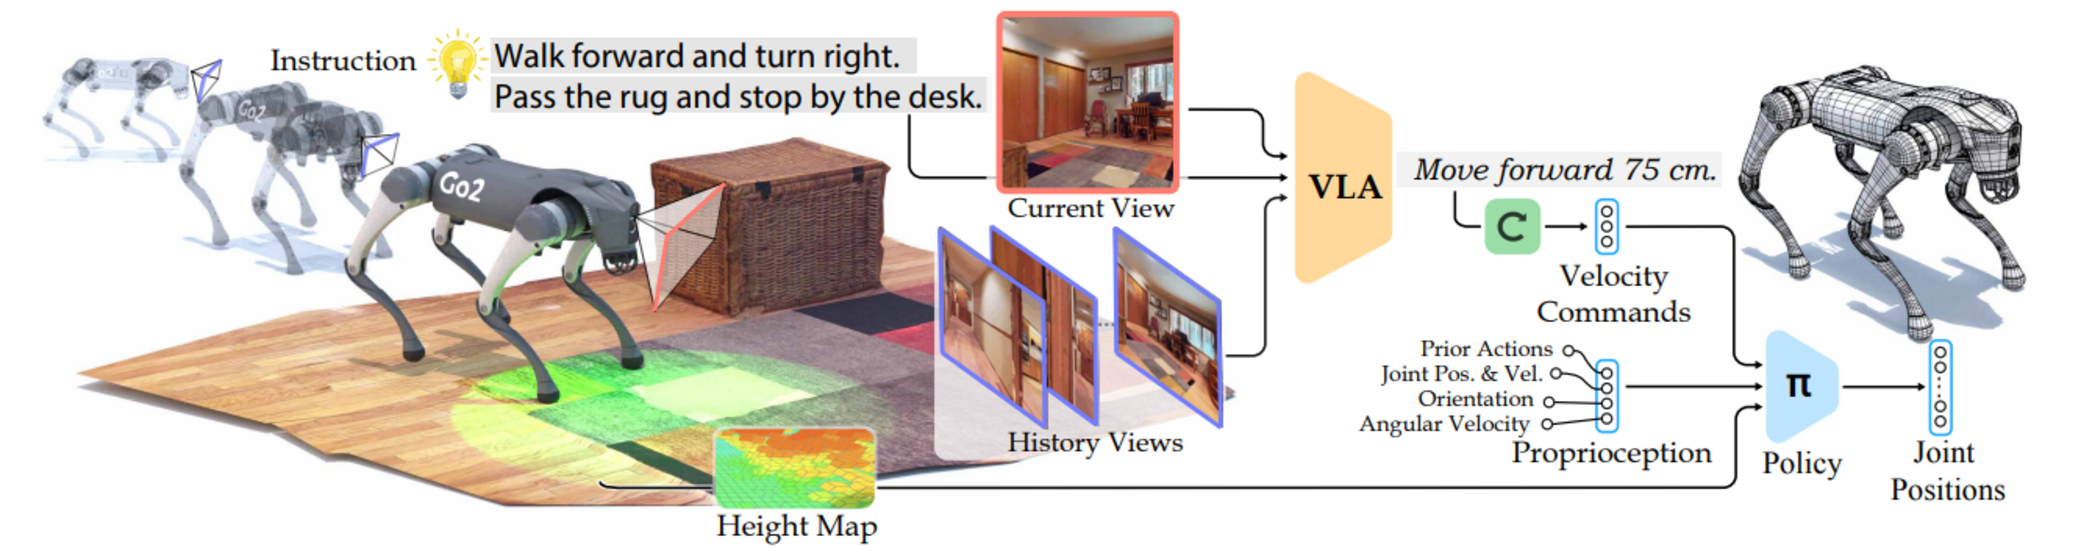
\includegraphics[width=\textwidth]{figs/2/navila_model.pdf}
  \caption{NaVILAの構造 (\cite{NaVILA_paper}より引用)}
  \label{fig:navila_model}
\end{figure}


NaVILA では，VLA が低レベル関節指令を直接出力するのではなく，
「前進 75\,cm」「右に 30 度回転」といった\textbf{中間表現を言語形式で生成}し，
低位の visual locomotion policy がそれを速度コマンド等へ変換して実行する．
この設計には，以下の利点がある \cite{NaVILA_paper}：
\begin{enumerate}[label=(\roman*)]
  \item 低位方策を入れ替えることで，同一のVLAを異なるロボットへ適用しやすい．
  \item 行動を言語として表現することで，多様な学習データ（実動画や推論QA等）を取り込みやすく，
        特定の低レベルコマンドへの過度な過学習を抑えながら推論能力を強化できる．
  \item 大規模 VLM は低頻度で高位の命令生成を行い，低位方策は実時間で高頻度に動作する．
\end{enumerate}


高位 VLA は画像ベースの VLM を用い，VLN において重要となる\textbf{履歴観測}と\textbf{現在観測}を役割に応じて区別する入力設計を採用する \cite{NaVILA_paper}．
具体的には，直近フレームを現在観測として扱い，それ以前のフレーム列を履歴（メモリ）としてサンプリングして同時に提示することで，
過去の行動の理解と次行動の決定を両立する．

低位の visual locomotion policy は Isaac Lab 上で強化学習（PPO）により学習され，
高位から与えられる中間表現を追従しつつ，障害物回避を含むロバストな歩行制御を獲得する \cite{NaVILA_paper}．
観測にはロボットの関節状態・姿勢に加え，LiDAR 点群から構成した height マップを用いることで，
強い日光や透明物体など視覚センサが不安定な条件でも安全な移動を可能にする \cite{NaVILA_paper}．

また学習時には Critic に特権情報を与える設計を取り入れ，実環境で利用可能な観測に基づく Actor を安定に学習する．

本研究では，NaVILAの二層構造のうち\textbf{低位方策（visual locomotion policy）}を基盤として採用し，
スタイル条件付けの対象となる歩行制御器として位置付ける．
